\documentclass[conference]{IEEEtran}

\usepackage[pdftex]{graphicx}
\graphicspath{{../pdf/}{../jpeg/}}
\usepackage[cmex10]{amsmath}
\usepackage[font=footnotesize]{subfig}

\usepackage{booktabs}
\usepackage{url}
\usepackage{listings}

\usepackage{color}
\definecolor{gray}{rgb}{0.4,0.4,0.4}
\definecolor{darkblue}{rgb}{0.0,0.0,0.6}
\definecolor{cyan}{rgb}{0.0,0.6,0.6}

\lstset{
  basicstyle=\ttfamily,
  columns=fullflexible,
  showstringspaces=false,
  commentstyle=\color{gray}\upshape
}

\lstdefinelanguage{XML}
{
  morestring=[b]",
  morestring=[s]{>}{<},
  morecomment=[s]{<?}{?>},
  stringstyle=\color{black},
  identifierstyle=\color{darkblue},
  keywordstyle=\color{cyan},
  morekeywords={xmlns,version,type}% list your attributes here
}

\begin{document}
\title{Java Call Graphs of the Hibernate-orm Repository}


\author{\IEEEauthorblockN{Adrian Schr{\"o}ter}
\IEEEauthorblockA{University of Victoria, Canada\\
schadr@acm.org}
\and
\IEEEauthorblockN{Jordan Ell}
\IEEEauthorblockA{University of Victoria, Canada\\
jell@uvic.ca}\and
\IEEEauthorblockN{Braden Simpson}
\IEEEauthorblockA{University of Victoria, Canada\\
braden@uvic.ca}\and
\IEEEauthorblockN{Triet Huynh}
\IEEEauthorblockA{University of Victoria, Canada\\
infiro@uvic.ca}\and
\IEEEauthorblockN{Daniela Damian}
\IEEEauthorblockA{University of Victoria, Canada\\
danielad@cs.uvic.ca}}

\maketitle


\begin{abstract}
This paper details call graphs extracted from Hibernate-orm using the Java Depndency Extractor.
We extracted call graphs at each of Hibernate-orm and provided both an XML file and a PostGreSQL database dump for other researchers to use.
We explained both the reasoning why we provided call graph information as well as what the call graphs we extracted do and do not contain.
All the data we presented in this paper is available at \url{home.segal.uvic.ca/~schadr/research-data/}.
\end{abstract}

\IEEEpeerreviewmaketitle

\section{Introduction}
Call graphs are used in various research projects that deal with assessing the quality of the software engineering projects such as failure predicting and effort estimation.
Several researchers have shown the value that call graphs can provide in assessing the complexity of a software project which in turn helps to improve on quality and productivity issues.

Although creating call graphs is considered part of static analysis, when not dealing with points to analysis or resolving issues related to polymorphism, generating call graphs for a single project over all its version can be very time consuming.
We found that extracting all call graphs for each of the more than 5000 commits to the mid sized Hibernate-orm project using a quad-core computer with a raid configuration takes several days.
This time other wise spend in procuring data can be better spend designing experiments and analyzing the data.

Thus with this paper we present a data set containing call graphs for each commit to the Hibernate-orm project in two date formats XML and PostGreSQL which we elicited on our blog\footnote{\url{adrian-schroeter.com/2012/10/09/what-is-your-favorite-data-format}}.
Both data sets are available at \url{home.segal.uvic.ca/~schadr/research-data/} and you can the find the tool we developed to extract the data at \url{www.github.com/schadr/java-dependency-extractor}.

%\textbf{Lorem ipsum dolor sit amet, consectetur adipiscing elit. Sed a quam nibh, eget dignissim odio. Maecenas euismod turpis et eros blandit vel ultrices leo aliquet. Duis laoreet metus id erat volutpat tincidunt. Integer velit neque, pharetra nec venenatis et, placerat non dui. Integer sagittis rutrum ligula at sodales. Phasellus eleifend vulputate tempus. Vivamus lacinia orci vulputate libero tincidunt non faucibus dui rutrum. Nam elementum ultrices scelerisque. Phasellus id magna erat. Duis mauris diam, pharetra eget accumsan eu, mollis vitae leo. Suspendisse porttitor, lacus eu blandit dictum, sem mauris semper sem, at venenatis velit ligula vel augue. Sed in metus sem.}
%
%\textbf{Sed ornare dui in mauris faucibus viverra. In hac habitasse platea dictumst. Cum sociis natoque penatibus et magnis dis parturient montes, nascetur ridiculus mus. Etiam tempus felis vitae nulla aliquet fringilla. Duis id arcu erat, nec mattis dolor. Morbi convallis lectus in augue bibendum eget ornare nunc laoreet. Morbi sagittis pulvinar neque, sit amet laoreet leo volutpat nec. Nullam congue, metus vitae accumsan scelerisque, urna diam sollicitudin felis, vitae varius urna erat sit amet justo. Donec quam metus, tristique quis sollicitudin nec, pulvinar in justo.}

In the remainder of this paper we will start with motivating the need for call graph data (Section~\ref{sec:need}).
Followed by what the call graphs we provide in our data set contain and what they omit (Section~\ref{sec:cg}).
In Section~\ref{sec:tool} describes the tool that we used to extract the data.
Next, we quickly summarize the Hibernate-orm project (Section~\ref{sec:orm}) followed by a description of the data formats we provide our data set in (Section~\ref{sec:df}).
We end the paper by discussing some potential data quality issues and future work in Sections~\ref{sec:issue} and~\ref{sec:fw}, respectively.

\section{The need for Call Graph data}
\label{sec:need}
Several research studies explore the effect of source code dependencies on other aspects of software development such as quality and productivity.

For example dependencies among software artifacts such as source code files or binaries are used to predict the likelihood of the artifacts of interest to contain one or more failures.
For example, Zimmermann et al~\cite{zimmermann:icse:2008} used call dependencies among individual artifacts to predict their failure likelihood and later extended that approach to account for the dependency network constructed by the artifacts of interests and the dependent artifacts~\cite{zimmermann:esem:2009}.

Other researchers constructed network among artifacts using simpler dependency metric such as co-changed files~\cite{pinzger:fse:2008} and used them to predict failures in artifacts.
Meneely at all used similar dependencies among software artifacts to construct networks of developers to predict failure likelihood in files~\cite{meneely:fse:2008}.
Using the same dependency metric combined with social interactions among developers Kwan et al~\cite{kwan:tse:2011} investigated the influence of the match between the technical dependencies connecting developers and their social interactions on build outcome.

This match between technical and social dimensions in software development is often referred to as socio-technical congruence.
Cataldo et al~\cite{cataldo:cscw:2006} in their seminal work used technical dependencies among developer that changed the same file for a given modification request and that networks match to social interactions constructed from social interactions among the same network's actors to related to performance metrics in the form of modification requests resolution time.
The correlation they uncovered sparked other researchers to peruse this line of work by creating tools to support developers by making those dependencies explicit~\cite{trainer2005:ariadne,sarma:icse:2009}.

We believe research that did use different dependency measure between code artifacts could have greatly benefited by adding call dependencies, either by improving their results or by enabling the researchers a better baseline comparison to evaluate the quality of their models.




\section{Call Graphs}
\label{sec:cg}
Wikipedia defines a call graph in the following way:
\emph{``A call graph ... is a directed graph that represents calling relationships between subroutines in a computer program.''}\footnote{en.wikipedia.org/wiki/Call\_graph}.
In this section we will not describe what a call graph is but focus on what the call graphs we provide in our data set do and do not contain.

\subsection{What is part of the Call Graph?}
The call graphs we provide with our data set are limited to method interactions as they are expressed in the source code.
Thus method interactions in the call graph are based on static analysis which excludes a points to analysis.
Instead of linking all possible methods that could be called we only express the direct connection.
For example, in Java a method might only be dealing with an Interface in which case we will create a link to the method as defined in the Interface rather than linking to all possible implementation of the interface.
Besides detailing for each commit to a source code repository the call graph by listing all methods defined in the source code as well as listing all methods called from each method we annotate each method whether it was changed.

\subsection{What is NOT port of the Call Graph?}
Since we rely on static analysis tools, as aforementioned we do not include all possible methods that could be called at runtime.
Furthermore, we limited ourselves to provide only information relevant to contracting a call graph.
Thus we did not include information that describe the different commits such as information about the commit author nor do we include the commit comment or links to issue trackers.
We also do not provide information about the project structure and the source code files.



\section{Java Dependency Extractor}
\label{sec:tool}
To extract the call graphs from a source code archive we created a java program available at \url{www.github.com/schadr/java-dependency-extractor}\footnote{\url{www.github.com/schadr/java-dependency-extractor}}.
This program extracts call graphs for each commit of a java project.
In order to avoid to rely on byte code we build on top of the Eclipse JDT compiler\footnote{www.eclipse.org/jdt/}.

This allows to create abstract syntax trees (ASTs) for each java file in the project.
The Eclipse JDT allows to resolve all code bindings that are possible given the source code and the available jars.
Note that resolves each file individually will result in a large amount of heap space required, thus it is preferable to parse all files together.

The version of the Java Dependency Extractor checks-out each version proceeds in four steps:
\begin{enumerate}
\item Check out version from the repository.
\item Create ASTs for all java files.
\item Visit all AST's to generate call graph.
\item Store the call graph.
\end{enumerate}
We apply those steps for all changes committed to a GIT repository.

\section{Hibernate-orm}
\label{sec:orm}
``\emph{Hibernate is concerned with helping your application to achieve persistence.  So what is persistence?  Persistence simply means that we would like our application's data to outlive the applications process.  In Java terms, we would like the state of (some of) our objects to live beyond the scope of the JVM so that the same state is available later.}''\footnote{\url{www.hibernate.org/about/orm} lasted visited October 18th, 2012}
The ORM component in particular implements Object/Relational Mapping to enable the efficient storage of Objects in a defined relational database scheme.

The Hibernate-orm git repository contains 5632 commits with the first commit June 2007 to the initial SVN repository which was moved to git in October 2010 and is now hosted on \url{github.com/hibernate/hibernate-orm}.

We chose Hibernate-orm for two reasons:
\begin{itemize}
\item It is publicly available on \url{github.com/hibernate/hibernate-orm}.
\item The issues tracker is also available and accessible via REST API at \url{hibernate.onjira.com/secure/Dashboard.jspa}.
\end{itemize}
This enables other researchers to combine the data we provide with other data sources such as issue tracker or other information that can be extracted from source code archives.


\begin{figure*}[t!]
\centering
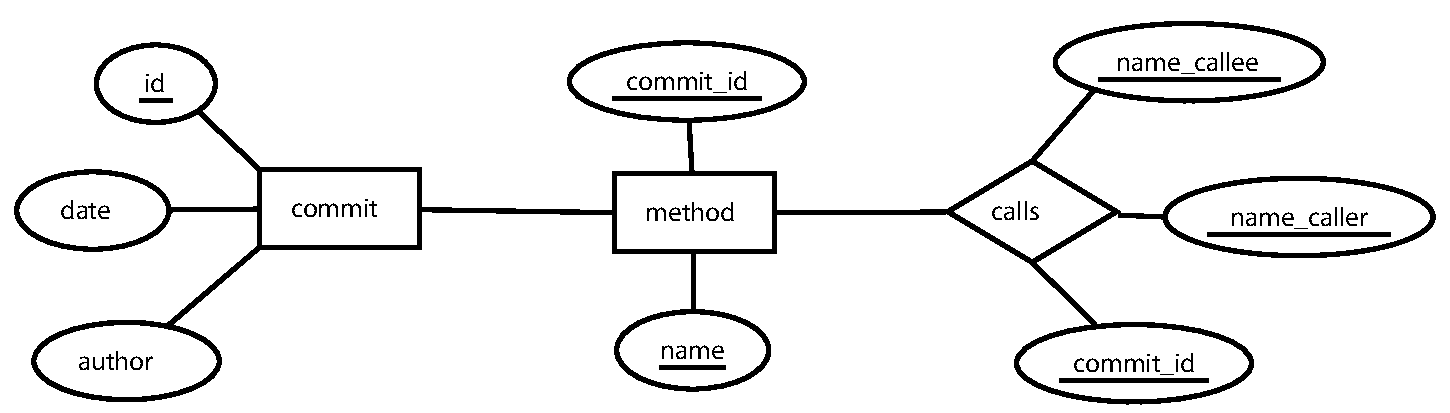
\includegraphics[width=\textwidth]{er}
\caption{PostGreSQL tables containing the Call Graph information.}
\label{er}
\end{figure*}

\begin{figure*}[th!]
\lstset{language=XML}
\begin{lstlisting}
<?xml version="1.0" encoding="utf-8"?>
<xs:schema xmlns:xs="www.w3.org/2001/XMLSchema">
  <xs:element name="project" type="projectType" maxOccurs="1" minOccurs="1" />

  <xs:complexType name="projectType">
    <xs:attribute name="name" type="xs:string" use="required" />
    <xs:element name="commit" type="commitType" />
  </xs:complexType>

  <xs:complexType name="commitType">
    <xs:attribute name="commit_id" type="xs:string" use="required" />
    <xs:attribute name="author" type="xs:string" use="required" />
    <xs:attribute name="time" type="xs:string" use="required" />
    <xs:element name="method" type="methodType" />     
  </xs:complexType>

  <xs:complexType name="methodType">
    <xs:attribute name="name" type="xs:string" use="required" use="required" />
    <xs:attribute name="was_changed" type="boolean" use="required" use="required" />
    <xs:element name="called_methods" type="calledMethodsType" />
  </xs:complexType>
  
  <xs:complexType name="calledMethodsType">
    <xs:attribute name="count" type="xs:integer" use="required" />
    <xs:element name="called_method" type="calledMethodType" />
  </xs:complexType>
  
  <xs:complexType name="calledMethodType">
    <xs:attribute name="name" type="xs:string" use="required" />
  </xs:complexType>

</xs:schema>
\end{lstlisting}
\caption{XML schema describing the data format of call graphs stored as XML.}
\label{list:xml:schema}
\end{figure*}



\section{Data Format}
\label{sec:df}
We provide out data in two formats: a XML\footnote{en.wikipedia.org/wiki/XML} file and a PostGreSQL\footnote{www.postgresql.org/} dump.
The data is available on 
\url{home.segal.uvic.ca/~schadr/research-data/}.

\subsection{XML}
The XML available at
\url{home.segal.uvic.ca/~schadr/research-data/hibernate-orm.dec2012.xml.gz}
conforming to the XML schema showin in Listing~\ref{list:xml:schema}.
The schema contains call-graph information for each commit detailing the commit id, the commit author, and the commit date.
The commit id can be used to retrieve the actual commit from the git repository.

Each commit entry contains the methods that were present in the version of that commit marked with whether a method was changed for that commit.
Each method listed in a commit contains a list of methods that are called.
The method name is fully qualified con sting of the package name, the class name, the method name, as well as a concatenation of the parameter types of the method.
For example:
\begin{lstlisting}
my.package.classA.methodB~int~String
\end{lstlisting}

The XML file available has an uncompressed size of XXgb and a compressed size of XXgb.

\subsection{PostGreSQL database}
The PostGreSQL dump is available at 
\url{home.segal.uvic.ca/~schadr/research-data/hibernate-orm.dec2012.psql.gz} and contains the tables modelled in the ER diagram shown in Figure~\ref{er}.

The ER diagram consist of three tables: 
(1) the commit table containing information about the individual commit, such as the commit id, the commit author, and the time of the commit.
(2) The method table contains information about the methods that were present in the version of the code at the given commit.
The method name is fully qualified con sting of the package name, the class name, the method name, as well as a concatenation of the parameter types of the method.
For example:
\begin{lstlisting}
my.package.classA.methodB~int~String
\end{lstlisting}
(3) The Calls table contains the information in what commit which method called which other method by containing the commit id, the calling method name, and the called method name.

The PostGreSQL database dump has a size of XXgb.


\section{Potential Data Quality Issues}
\label{sec:issue}
Due to the size of the data set we only could do random spot checks of the correctness of the data.
There are several issues:
\begin{itemize}
\item The Eclipse compiler is not able to resolve every binding due to missing jars and packaging issues.
\item The project might contain files representing the same classes belonging to the same package which can lead to either the same method name being listed multiple times as well as a method containing more called methods that are actually present in the source code for any given class implementation.
\end{itemize}


\section{Future Work}
\label{sec:fw}
Our future work is two fold:
(1) Offer call graph data for more projects and
(2) add more type of dependencies.
To enable us to extract call graphs from more projects is straight forward as it mainly involves simply running out tool on other projects.

Adding more dependencies is more challenging as this involves further analysis of the source code.
Other dependency types that we are considering in supporting are:
\begin{itemize}
\item Data dependencies connecting methods and classes through the usage of the same variables.
\item Points to dependencies linking methods that could be called using polymorphism.
\end{itemize}

We are always looking for contributors to the Java Dependency Extractor, if you are interested in supporting this project please send and email to schadr@acm.org or fork and create a pull request on github.com.



\bibliographystyle{IEEEtran}
\bibliography{bib}

\end{document}


